\documentclass{beamer}

\usepackage{beamerthemesplit}
\usepackage{verbatim}
\usepackage[normalem]{ulem}

\usepackage{xcolor}

\usepackage{hyperref}

\definecolor{gold}{rgb}{1.,0.84,0.}
\definecolor{brightred}{rgb}{1.,0.4,0.4}
\definecolor{mygray}{RGB}{200,200,200}
\definecolor{lightsteelblue}{RGB}{176,196,222}
\definecolor{lightskyblue}{RGB}{135,206,250}
\definecolor{cadetblue}{RGB}{95,158,160}

\usetheme{default}
\usecolortheme{mule}

\usefonttheme{serif}

%\DeclareGraphicsExtensions{.pdf,.png,.jpg}

\newcommand{\mcal}{\textsc{metacalibration}}
\newcommand{\Mcal}{\textsc{Metacalibration}}

\newcommand{\mcalR}{\mbox{\boldmath $R$}}
\newcommand{\mcalRscalar}{\mbox{$R$}}

\newcommand{\mcalRmean}{\mbox{\boldmath $\langle R \rangle$}}
\newcommand{\mcalRscalarmean}{\mbox{$\langle R \rangle$}}

\newcommand{\mcalRpsf}{$R^{p}$}
\newcommand{\mcalRpsfnoise}{$R^{p}_\eta$}
\newcommand{\mcalRo}{\mbox{\boldmath $R_o$}}
\newcommand{\mcalRnoise}{\mbox{\boldmath $R_\eta$}}

\newcommand{\mcalRmeanalpha}{\mbox{\boldmath $\langle R_\alpha \rangle$}}
\newcommand{\mcalRmeanbeta}{\mbox{\boldmath $\langle R_\beta \rangle$}}

\newcommand{\mcalRg}{\mbox{\boldmath $R_\gamma$}}
\newcommand{\mcalRS}{\mbox{\boldmath $R_S$}}
\newcommand{\mcalRgmean}{\mbox{\boldmath $\langle R_\gamma \rangle$}}
\newcommand{\mcalRSmean}{\mbox{\boldmath $\langle R_S \rangle$}}

\newcommand{\mcalRtwopt}{\mbox{\boldmath $R^{2pt}$}}
\newcommand{\mcalRtwoptmean}{\mbox{\boldmath $\langle R^{2pt} \rangle$}}


\newcommand{\mcalRmodel}{\mbox{\boldmath $R^{model}$}}
\newcommand{\mcalRnoisemodel}{\mbox{\boldmath $R^{model}_\eta$}}


\newcommand{\vecg}{\mbox{\boldmath $\gamma$}}
\newcommand{\vest}{\mbox{\boldmath $e$}}

\newcommand{\snr}{$S/N$}
\newcommand{\snT}{$(S/N)_{\textrm{size}}$}
%\newcommand{\snT}{$\left( \frac{S}{N}\right)_{\textrm{size}}$}
\newcommand{\snflux}{$(S/N)_{\textrm{flux}}$}
%\newcommand{\snflux}{$\left( \frac{S}{N}\right)_{\textrm{flux}}$}

\newcommand{\lensfit}{\texttt{LENSFIT}}
\newcommand{\numba}{\texttt{Numba}}
\newcommand{\python}{\texttt{Python}}
\newcommand{\ngmix}{\texttt{ngmix}}
\newcommand{\shear}{{\bf g}}
\newcommand{\redmapper}{redMaPPer}
\newcommand{\est}{$e$}


\newcommand{\prelim}{{\bf{\it Preliminary}}}

\newcommand{\uberseg}{{\"u}berseg}


\title{Erin Sheldon: Dark Energy Survey and LSST}
\author{Erin Sheldon}
\institute{Brookhaven National Laboratory}

% http://texblog.net/latex-archive/plaintex/beamer-footline-frame-number/
% to add the page (frame ) number and not screw up the bottom line
% works for split themes?
\expandafter\def\expandafter\insertshorttitle\expandafter{%
      \insertshorttitle\hfill%
        \insertframenumber\,/\,\inserttotalframenumber}

% suppress navigation bar
\beamertemplatenavigationsymbolsempty
\setbeamertemplate{footline}{}

\begin{document}


%\frame{\titlepage}

\setbeamerfont*{itemize/enumerate body}{size=\Large}
\setbeamerfont*{itemize/enumerate subbody}{parent=itemize/enumerate body}
\setbeamerfont*{itemize/enumerate subsubbody}{parent=itemize/enumerate body}



\frame
{
    \frametitle{Erin Sheldon: Dark Energy Survey and LSST}

    \setbeamerfont*{itemize/enumerate body}{size=\normalsize}

    \begin{itemize}

        \item Dark Energy Survey (DES)
            \begin{itemize}
                \item Imaging survey, goal to measure the properties of dark energy
                \item Primary probe is weak gravitational lensing
                \item Just released cosmology results for year 1 out of 5
                \item Sheldon performed weak lensing shear measurements
                \item Sheldon {\color{gold} Co-coordinator of Shear Measurement Working Group}
            \end{itemize}

        \item LSST
             \begin{itemize}
                \item Imaging survey, goal to measure the properties of dark energy
                \item Primary probe is weak gravitational lensing
                \item In building phase
                \item Sheldon {\color{gold} Shear Measurement Project Coordinator} in LSST Dark Energy Science Collaboration (DESC)
            \end{itemize}

    \end{itemize}

}

\frame
{
    \frametitle{DES Year 1 Cosmology Results}

    \setbeamerfont*{itemize/enumerate body}{size=\normalsize}

    \begin{columns}
        \begin{column}{0.5\textwidth}
            \begin{itemize}

                \item DES measures mean ($\Omega_m$) and variance ($\sigma_8$) of the mass density
                    in the universe

                \item Best constraints from lensing to date

                \item Also measures equation of state of dark energy, ratio
                    of pressure to density: $w = p/\rho$

                \item Combine with cosmic microwave background experiment Planck


            \end{itemize}
        \end{column}
        \begin{column}{0.5\textwidth}
            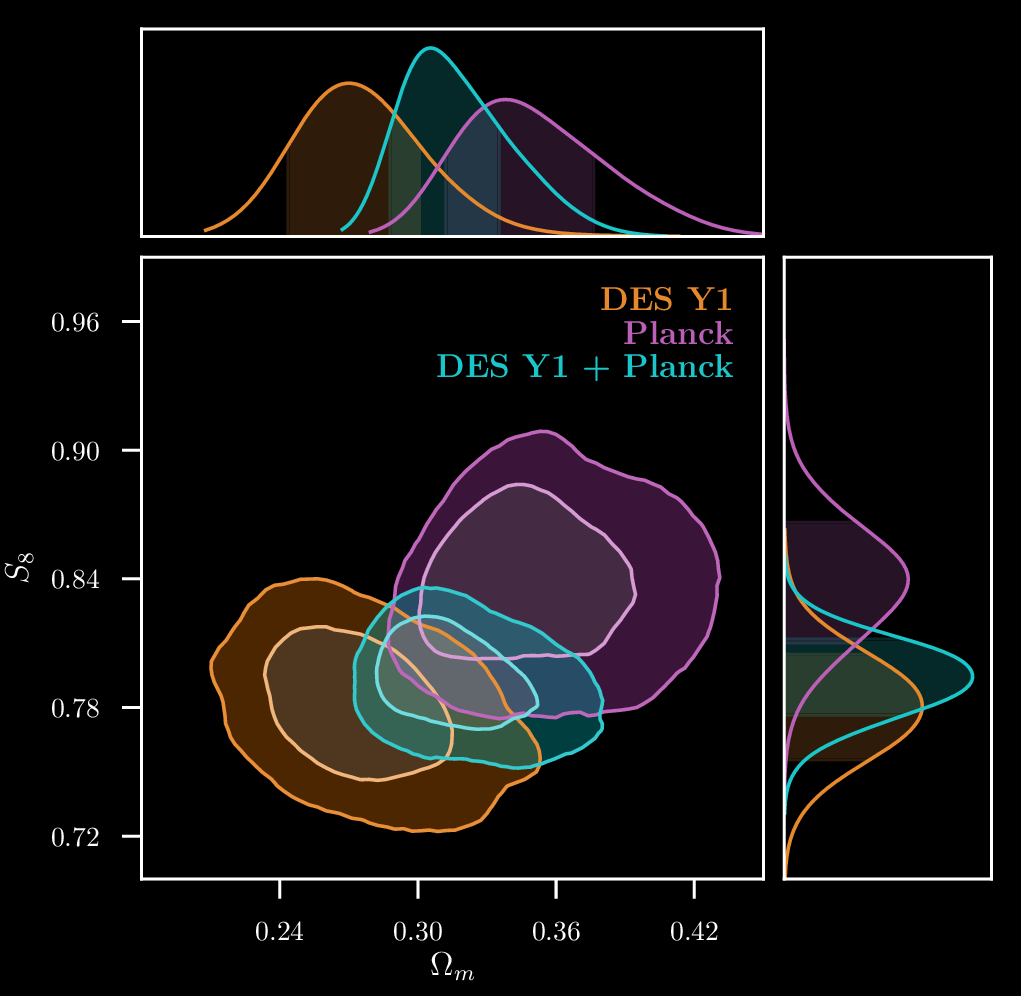
\includegraphics[width=\textwidth]{dpnl_l_inv.png}
            \newline
            {\tiny Mass density and $S_8 = \sigma_8 (\Omega_m/0.3)^{0.5}$}
        \end{column}
    \end{columns}
}

\frame
{
    \frametitle{DES Year 1 Cosmology Results: Constraints on $w$}

    \setbeamerfont*{itemize/enumerate body}{size=\normalsize}

    \begin{center}
        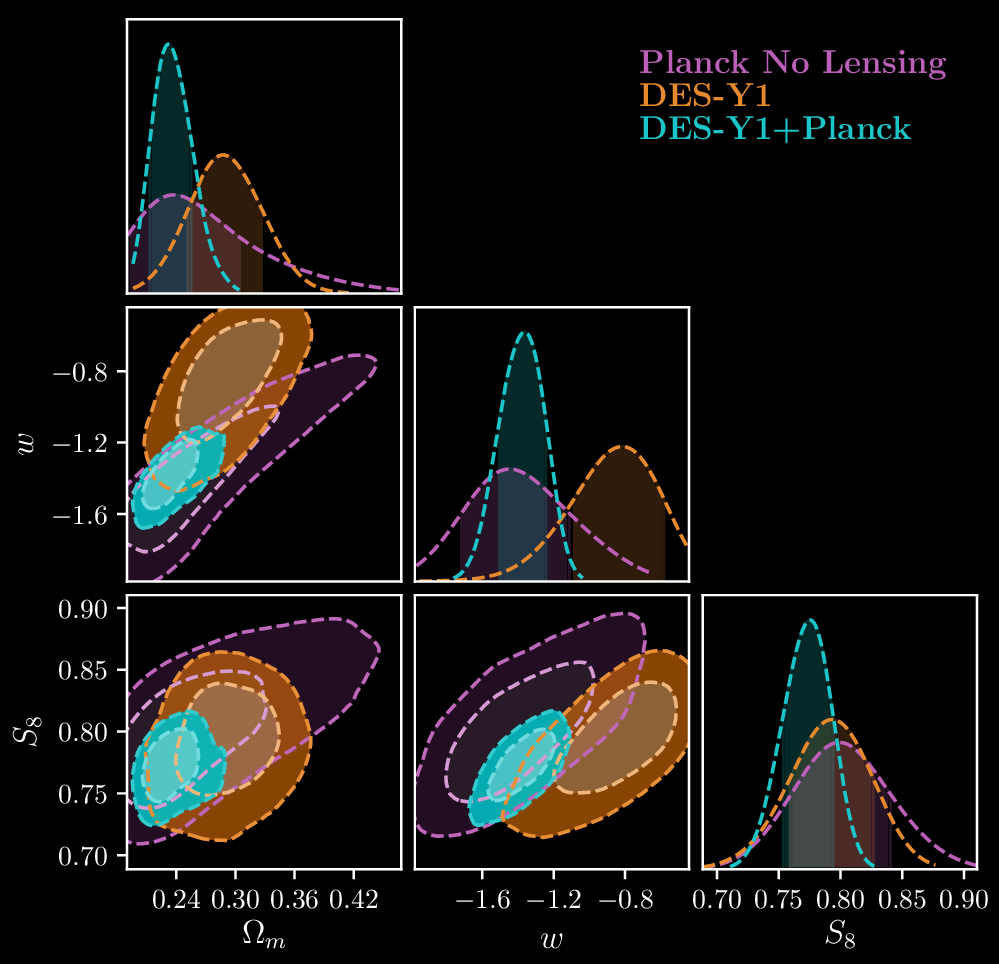
\includegraphics[width=0.65\textwidth]{dpnl_w_inv.png}
        \newline
        Constraints on mass density, variance, and dark energy equation of state $w$
    \end{center}

}

\frame
{
    \frametitle{LSST Work}

    \setbeamerfont*{itemize/enumerate body}{size=\normalsize}

    \begin{itemize}

         \item Sheldon {\color{gold} Shear Measurement Project Coordinator} in
             LSST Dark Energy Science Collaboration (DESC)

             \begin{itemize}
                 \item Weak lensing shear is the primary dark energy probe for LSST.
                 \item The success of the project hinges on these basic measurements.
             \end{itemize}

         \item Currently porting DES weak lensing and photometry codes to work
             with LSST data management (DM) products

         \begin{itemize}
             \item Stress test:  Goal to run on DM outputs created for the Hyper
                 Suprime Camera survey

             \item Good test of our readiness, but also opportunity for new science
                 to come out of DESC in preparation for LSST commissioning
         \end{itemize}

    \end{itemize}



}





\end{document}
